\section{10.1 The Macroscopization of Quantum Teleportation}

\begin{quote}
``Why accelerate a spaceship weighing thousands of tons to light speed? That is an enormous waste of energy. What really matters is not the atoms of the spaceship, but the arrangement of atoms---that is, information. If you can extract the information of a spaceship, you don't need to transport it; you just need to `print' it at the destination. The universe is not a logistics company; the universe is a fax machine.''
\end{quote}

\begin{figure}[htbp]
\centering
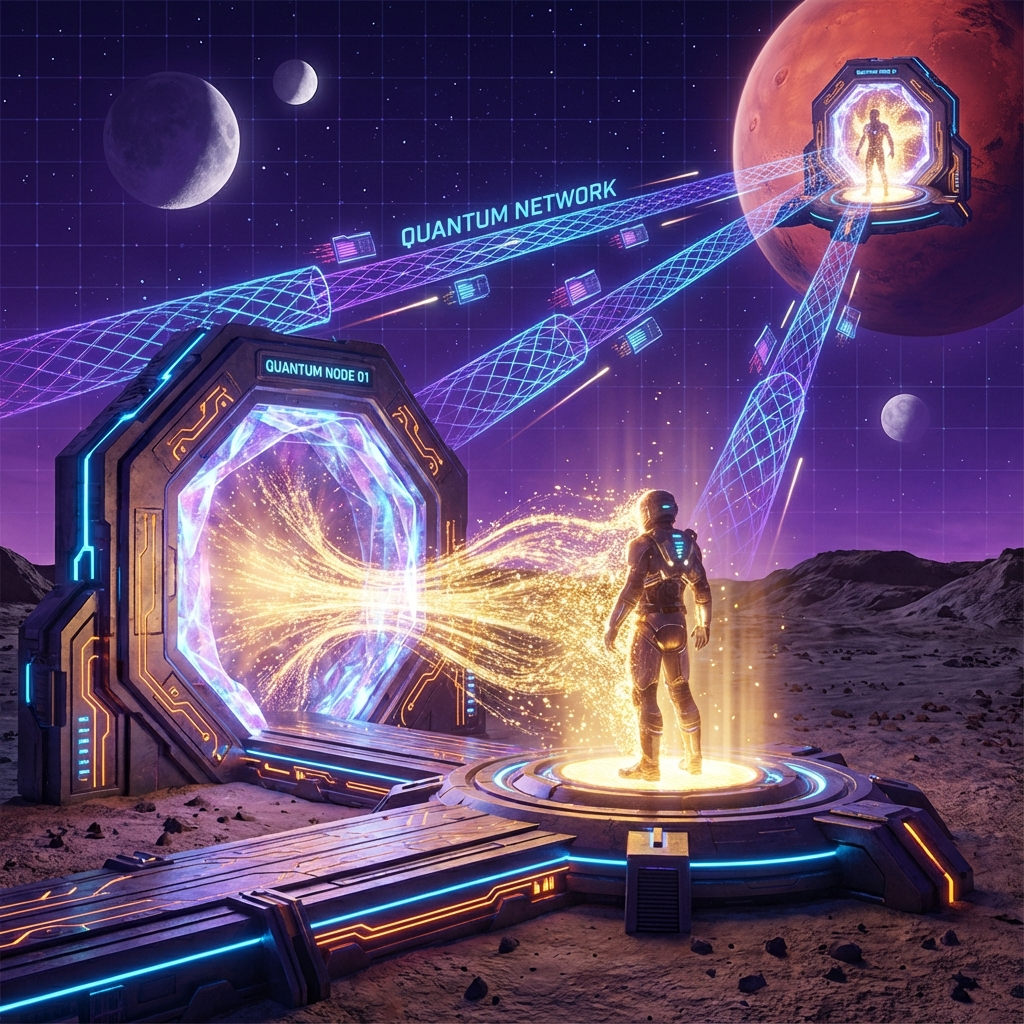
\includegraphics[width=0.8\textwidth]{assets/chapter-10/10-01-01-quantum-teleportation.png}
\caption{Quantum Teleportation}
\label{fig:quantum-teleportation}
\end{figure}

\subsection{Abandoning $v_{ext}$, Embracing $v_{int}$}

In traditional astronautics, we are obsessed with \textbf{$v_{ext}$ (external velocity)}. We build rockets and engines, trying to push matter lumps as fast as possible.

But this faces the iron wall of relativity: the larger the mass, the harder to accelerate, and it can never reach light speed.

\textbf{Quantum teleportation} provides a completely different approach:

Abandon moving matter ($v_{ext}$), and instead move \textbf{structure ($v_{int}$)}.

\begin{itemize}
\item \textbf{Principle}: According to quantum mechanics, all physical properties of a particle (spin, polarization, energy state) can be completely extracted and transferred to another particle, as long as they share \textbf{entanglement}.

\item \textbf{Operation}:

    \begin{enumerate}
    \item \textbf{Entanglement resource}: Establish a pair of shared Bell-state particles between Earth (A) and Mars (B).

    \item \textbf{Bell measurement}: At A, perform joint measurement on the particle to be teleported and the entangled particle.

    \item \textbf{Collapse and transmission}: The particle at A instantly collapses (original destroyed). Measurement results (classical two-bit information) are sent to B via radio.

    \item \textbf{Unitary reconstruction}: After B receives the information, perform corresponding rotation operations on the entangled particle here. A miracle happens: the particle at B instantly becomes the particle that was originally at A.
    \end{enumerate}
\end{itemize}

\textbf{Note:} No matter has traveled the distance from Earth to Mars.

The ``blank paper'' (original particle) originally at B is written with ``ink'' (quantum state) from A.

Geometrically, this is equivalent to A and B undergoing \textbf{``topological coincidence''} in Hilbert space.

\subsection{The Challenge of Macroscopization: The Avalanche of Information}

This protocol has been experimentally successful for single photons. But to teleport a person or a spaceship, we need \textbf{macroscopization}.

A person contains approximately $10^{28}$ atoms. Each atom has a quantum state.

To teleport a person, we need:

\begin{enumerate}
\item \textbf{Prepare $10^{28}$ pairs of entangled particles}: This requires enormous quantum memory.

\item \textbf{Perform $10^{28}$ Bell measurements}: This requires extremely high-precision scanners.

\item \textbf{Transmit $2 \times 10^{28}$ bits of classical information}: This requires extremely high bandwidth.
\end{enumerate}

This sounds difficult, but it is a \textbf{``linear problem''}, not a physical \textbf{``exponential problem''}.

As $c(\tau)$ (light speed/computational power) grows exponentially, bandwidth and storage will eventually not be problems.

For Type III civilizations, scanning a person's data volume is as simple as scanning a QR code for us now.

\subsection{Cut and Paste: The Cost of No-Cloning}

The greatest ethical and ontological impact of macroscopic teleportation comes from the \textbf{No-Cloning Theorem}.

Quantum mechanics forbids perfect copying. This means that to complete teleportation, \textbf{the original must be destroyed}.

\begin{itemize}
\item At the moment of scanning, the measurement operation destroys the quantum states of all atoms in your body.

\item You on Earth \textbf{``evaporate''} in this process, becoming a pile of chaotic hot gas.

\item And you on Mars, at the same instant, \textbf{``reconstruct''} using the received data.
\end{itemize}

\textbf{Is this travel, or suicide followed by rebirth?}

From the perspective of \textbf{Vector Cosmology}, because \textbf{``memory is ontology''}, as long as the geometric structure of $v_{int}$ (consciousness/memory/personality) is transferred losslessly, this is \textbf{the same you}.

\begin{itemize}
\item \textbf{Material carrier} (carbon atoms) is just consumables.

\item \textbf{Topological structure} (wave function) is the soul.
\end{itemize}

You did not die; you just changed decks, but played the same straight flush.

\subsection{Conclusion: Distance is ``Formatted''}

When macroscopic teleportation becomes everyday technology, the \textbf{topological structure} of the universe is completely changed.

Space is no longer an obstacle.

\begin{itemize}
\item As long as you pre-deploy an \textbf{``entanglement receiving station''} (equivalent to a 3D printer) at the target location (e.g., Alpha Centauri), you can go there anytime.

\item Interstellar travel becomes \textbf{``data upload''}.

\item Distance $d$ no longer corresponds to time $t = d/v$, but to \textbf{bandwidth latency}.
\end{itemize}

\textbf{This is ``topological short-circuiting.''}

We no longer laboriously crawl across the surface of the spacetime fabric (following geodesics).

We directly use entanglement threads to tie a knot on the back of the fabric, \textbf{pinching} the starting point and endpoint together.

Since we can already teleport matter and consciousness through entanglement, what if we encounter the most extreme obstacles in the universe during transmission---such as black hole horizons or so-called ``firewalls''? Can this transmission still proceed?

Can we use this technology to ignore the one-way nature of horizons and directly jump into black hole interiors, even pass through them?

This leads to the theme of the next section: \textbf{Traversing Firewalls}. We will see how quantum error-correcting codes act as an ``invisibility cloak,'' protecting information security through spacetime fracture zones.

